% Chapter 10. The MCP Apps security contract, drawn as what is blocked.
\documentclass[tikz,border=6pt]{standalone}
% Shared look for every TikZ figure in the book.
% Colours match book/preamble.tex exactly. Change both or neither.

\usepackage{tikz}
\usepackage{xcolor}
\usepackage{amsmath}
\IfFileExists{libertinus.sty}{\usepackage[mono=false]{libertinus}}{}
\IfFileExists{inconsolata.sty}{\usepackage[varqu,varl,scaled=0.95]{inconsolata}}{}

\usetikzlibrary{
  arrows.meta, positioning, calc, fit, backgrounds, shapes.geometric,
  shapes.misc, decorations.pathreplacing, decorations.pathmorphing,
  patterns, chains, matrix, shadows.blur
}

\definecolor{ink}{HTML}{15181D}
\definecolor{muted}{HTML}{5B6472}
\definecolor{rule}{HTML}{C9CED6}
\definecolor{wash}{HTML}{F4F5F7}
\definecolor{accent}{HTML}{0F5C8C}
\definecolor{accentsoft}{HTML}{E7F0F6}
\definecolor{warm}{HTML}{B4531A}
\definecolor{warmsoft}{HTML}{FBF0E7}
\definecolor{good}{HTML}{2C6E49}
\definecolor{goodsoft}{HTML}{E9F2EC}
\definecolor{danger}{HTML}{9B2226}
\definecolor{dangersoft}{HTML}{FAECEC}

\tikzset{
  font=\sffamily\small,
  >={Stealth[length=5pt, width=4pt]},
  %
  box/.style={
    draw=rule, line width=0.8pt, fill=wash, rounded corners=2pt,
    inner sep=7pt, align=center, text=ink, minimum height=9mm,
  },
  boxa/.style={box, draw=accent, fill=accentsoft},
  boxg/.style={box, draw=good,   fill=goodsoft},
  boxw/.style={box, draw=warm,   fill=warmsoft},
  boxd/.style={box, draw=danger, fill=dangersoft},
  %
  lane/.style={draw=rule, line width=0.7pt, fill=white, rounded corners=2pt,
               inner sep=6pt, align=center, minimum width=26mm},
  %
  flow/.style={draw=accent, line width=1.0pt, ->},
  flowback/.style={flow, densely dashed},
  flowmuted/.style={draw=muted, line width=0.8pt, ->},
  lifeline/.style={draw=rule, line width=0.7pt, densely dotted},
  %
  lbl/.style={font=\sffamily\scriptsize, text=muted, inner sep=2pt},
  lblink/.style={font=\sffamily\scriptsize, text=ink, inner sep=2pt},
  tag/.style={font=\ttfamily\scriptsize, text=accent, inner sep=2pt,
              fill=white, inner xsep=3pt},
  note/.style={font=\sffamily\scriptsize\itshape, text=muted, align=left},
  %
  band/.style={draw=none, rounded corners=1pt},
  tick/.style={draw=muted, line width=0.6pt},
}

% A horizontal timeline bar segment: \barseg{x0}{x1}{y}{colour}{label}
\newcommand{\barseg}[5]{%
  \fill[#4, rounded corners=1pt] (#1,#3-0.16) rectangle (#2,#3+0.16);
  \node[lbl, text=white, font=\sffamily\scriptsize\bfseries]
       at ({(#1+#2)/2},#3) {#5};
}

\begin{document}
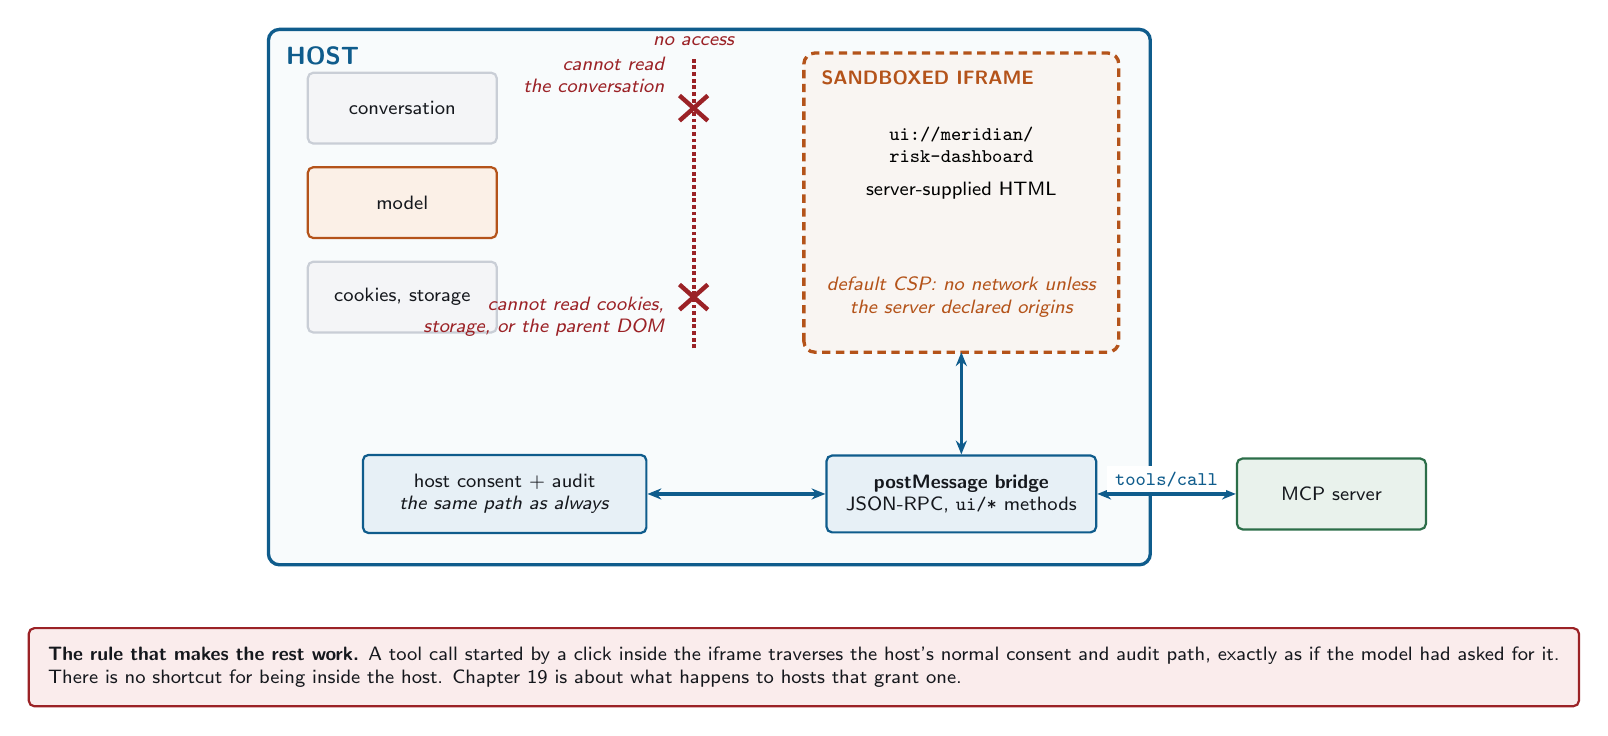
\begin{tikzpicture}[x=1cm, y=1cm]

  % --- host -------------------------------------------------------------
  \draw[draw=accent, line width=1.2pt, rounded corners=4pt,
        fill=accentsoft, fill opacity=0.28]
    (-0.8,-1.6) rectangle (10.4,5.2);
  \node[anchor=north west, font=\sffamily\bfseries\small, text=accent]
    at (-0.7,5.1) {HOST};

  \node[box, minimum width=24mm, font=\sffamily\scriptsize] (conv)    at (0.9,4.2) {conversation};
  \node[boxw, minimum width=24mm, font=\sffamily\scriptsize] (model)  at (0.9,3.0) {model};
  \node[box, minimum width=24mm, font=\sffamily\scriptsize] (cookies) at (0.9,1.8) {cookies, storage};

  % --- the iframe -------------------------------------------------------
  \draw[draw=warm, line width=1.2pt, densely dashed, rounded corners=4pt,
        fill=warmsoft, fill opacity=0.5]
    (6.0,1.1) rectangle (10.0,4.9);
  \node[anchor=north west, font=\sffamily\bfseries\scriptsize, text=warm]
    at (6.1,4.8) {SANDBOXED IFRAME};
  \node[align=center, font=\sffamily\scriptsize] at (8.0,3.5)
    {\texttt{ui://meridian/}\\\texttt{risk-dashboard}\\[4pt] server-supplied HTML};
  \node[note, text=warm, align=center] at (8.0,1.8)
    {default CSP: no network unless\\the server declared origins};

  % --- the barrier ------------------------------------------------------
  \draw[draw=danger, line width=1.4pt, densely dotted] (4.6,1.15) -- (4.6,4.85);
  \foreach \y in {4.2, 1.8} {
    \draw[draw=danger, line width=1.6pt] (4.42,\y-0.16) -- (4.78,\y+0.16);
    \draw[draw=danger, line width=1.6pt] (4.42,\y+0.16) -- (4.78,\y-0.16);
  }
  \node[note, text=danger, align=center] at (4.6,5.05) {no access};

  \node[note, text=danger, anchor=east, align=right] at (4.35,4.62)
    {cannot read\\the conversation};
  \node[note, text=danger, anchor=east, align=right] at (4.35,1.55)
    {cannot read cookies,\\storage, or the parent DOM};

  % --- the only channel -------------------------------------------------
  \node[boxa, minimum width=34mm, align=center, font=\sffamily\scriptsize]
    (bridge) at (8.0,-0.7)
    {\textbf{postMessage bridge}\\JSON-RPC, \texttt{ui/*} methods};
  \draw[<->, draw=accent, line width=1.2pt] (8.0,1.1) -- (bridge);

  \node[boxa, minimum width=36mm, align=center, font=\sffamily\scriptsize]
    (policy) at (2.2,-0.7)
    {host consent + audit\\\emph{the same path as always}};
  \draw[<->, draw=accent, line width=1.2pt] (bridge) -- (policy);

  \node[boxg, minimum width=24mm, font=\sffamily\scriptsize] (server) at (12.7,-0.7)
    {MCP server};
  \draw[<->, draw=accent, line width=1.2pt] (bridge)
    -- node[tag, above] {tools/call} (server);

  % --- the rule ---------------------------------------------------------
  \node[boxd, minimum width=150mm, align=left, font=\sffamily\scriptsize]
    at (6.0,-2.9)
    {\textbf{The rule that makes the rest work.} A tool call started by a click
     inside the iframe traverses the host's normal consent and audit path,
     exactly as if the model had asked for it.\\
     There is no shortcut for being inside the host. Chapter 19 is about what
     happens to hosts that grant one.};

\end{tikzpicture}
\end{document}
